\usetikzlibrary{arrows,shapes,snakes,automata,backgrounds,petri}
\tikzstyle{state}=[circle,thick,draw=black!75,fill=white!20,minimum size=6mm]

\chapter{SIR\label{chapter:sir}}
\lhead{SIR}
\begin{refsection}
\chapterauthor{Max Obrist und Martin Stypinski}

Die \emph{Epidemiologie} ist eine wissenschaftliche Disziplin, welche sich mit Ursache, Verbreitung und Folgen von gesundheitsbezogenen Ereignissen in einer Population befasst.
Im Gegensatz zur klassischen Medizin befasst sich die Epidemiologie nicht damit, wie eine Krankheit, bzw. eine kranke Person geheilt werden kann, sondern damit, wie sich eine spezielle Krankheit ausbreitet, und mit welchen Mitteln die Krankheit in der Gesamtbevölkerung besiegt werden kann.

Die \emph{mathematische Epidemiologie} -- womit wir uns in diesem Kapitel ansatzweise befassen -- ist ein Teilgebiet der Epidemiologie, sowie der \emph{theoretischen Biologie}.
Die mathematische Epidemiologie befasst sich speziell mit mathematischen Modellen zur Ausbreitung von Krankheiten, stellt also Fragen nach z.B. der Form oder der Ausbreitungsgeschwindigkeit von ansteckbaren Krankheiten, beispielsweise von Influenza, Masern oder auch Ebola. 
Das \emph{SIR-Model}, welches wir auf den nächsten Seiten detailliert anschauen werden, ist ein mathematisches Modell, mit welchem der Verlauf einer Krankheit in einer Population modelliert werden kann.

\section{Problemstellung}
Wir stellen uns vor, dass in einer Bevölkerungsgruppe eine Krankheit ausbricht. 
Es könnte sich dabei z.B. um einen neuen Influenza-Stamm handeln.
Bei einer Grippe wird ein Träger, nachdem er die Krankheit ausgestanden hat, bekanntermassen immun gegen diesen speziellen Stamm (Aber nicht gegen andere Stämme von Influenza).
Nachdem die Krankheit bereits ein wenig durch die Bevölkerung gegangen ist, lassen sich anhand der ersten Daten einige Informationen über die Krankheit erfassen.
Zum Beispiel kann herausgefunden, wie infektiös eine Krankheit ist, oder wie lange es nach einer Infektion durchschnittliche dauert, bis ein Träger die Infektion überstanden hat.

Anhand dieser Informationen soll nun ein Modell entwickelt werden, mit welchem gewisse Vorhersagen über den weiteren Verlauf der Krankheit getroffen werden können. 
Es soll nochmals wiederholt werden, dass mit dem Verlauf der Krankheit nicht der Verlauf der Krankheit in einem Individuum gemeint ist, sondern wie sich die Krankheit in der Bevölkerung selbst ausbreitet. 
Der Patient ist sozusagen also nicht ein einzelner Kranker, sondern eine ganze Population auf einmal.

Der Einfachheit halber nehmen wir an, dass die Grösse der Population konstant ist.
Die Geburten- und Sterberate in der Bevölkerung werden damit ignoriert.
Diese Annäherung ist dann möglich, wenn die Lebenserwartung (mehrere dutzend Jahre) im Vergleich zum Krankheitsverlauf (ein paar Wochen bis Monate) sehr gross ist.
In diesem Fall hat der Bevölkerungswachstum im Verlauf der Krankheit nur einen vergleichbar kleinen Einfluss auf die Population, und kann dadurch vernachlässigt werden.
Im Falle von langanhaltenden Krankheiten, z.B. HIV/AIDS, wo der Krankheitsverlauf mehrere Jahrzehnte dauern kann, müsste das Modell entsprechend erweitert werden.

\section{SIR-Modell}
Bei allen Krankheiten, welche sich wie die oben beschriebene Grippe verhalten -- Ein gesundes Subjekt wird infiziert, ist eine gewisse Zeit lang krank und ist nach der Genesung immun gegen den Erreger -- lässt sich die Bevölkerung in 3 Kompartimente aufteilen. Weitere klassische Beispiele für Krankheiten, die sich nach diesem Muster ausbreiten, sind die typischen Kinderkrankheiten Masern, Mumps oder Röteln.
\begin{description}
  \item [Susceptibles ($\mathbf{S}$)] sind Individuen, welche von einem Träger der Krankheit angesteckt werden können. Sie tragen die Krankheit weder in sich, noch sind sie bereits immun gegen dagegen. Werden sie angesteckt, werden sie zu \emph{Infected}.
  \item [Infected ($\mathbf{I}$)] sind Personen, die zum aktuellen Zeitpunkt mit der Krankheit infiziert sind, und auch andere Individuen infizieren können. Nach einer gewissen Zeit genesen sie, und verschieben sich dann in das Kompartiment \emph{Removed}.
  \item [Removed ($\mathbf{R}$)] sind jene Individuen, welche Immun gegen die Krankheit sind und nicht erneut angesteckt werden können. Im normalen SIR-Modell wird dabei nicht zwischen genesenen und verstorbenen Individuen unterschieden, weshalb dieses Kompartiment schlicht \emph{Removed} genannt wird.
\end{description}

Es wurde bereits erwähnt, dass davon ausgegangen wird, dass die Bevölkerung $N$ konstant ist, also $S + I + R = \text{const}$. Damit muss die Summe aller Ableitungen konstant sein, wie
\begin{align*}
  \frac{d}{dt}\left(S+I+R\right) = 0
\end{align*}
aufzeigt. 
$N$, sowie die die Kompartimente $S$, $I$ und $R$ können dabei sowohl die nummerische Grösse der Population beschreiben, oder aber sie beschreiben die Populationen relativ. 
In weiteren Verlauf wird zweiteres gewählt, damit ist zu jedem Zeitpunkt $N = 1$.
Das SIR-Modell beschreibt nun, wie genau sich eine Krankheit in der Bevölkerung ausbreitet, wie sich also die Individuen durch diese 3 Kompartimente bewegen.
Um dies zu beschreiben, muss bekannt sein, mit welchen Raten sich die Individuen zwischen den Kompartimenten verschieben.

\begin{figure}[H]
  \centering
  
    	 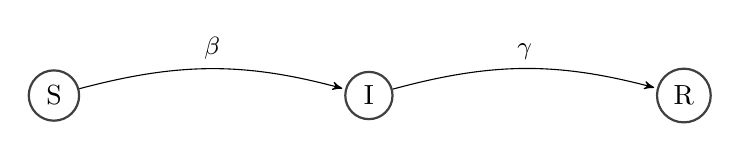
\begin{tikzpicture}[node distance=4cm,>=stealth',bend angle=15,auto]
    	   \begin{scope}
    	     % First net
    	     \node [state] (s1)                                    {S};
    	     \node [state] (s2) [right of=s1]                      {I};
    	     \node [state] (s3) [right of=s2]                      {R};
    	     	
         	\path[every node/.style={font=\sffamily\small}]
      	        (s1) edge [post, bend left] node {$\beta$} (s2)
      	        (s2) edge [post, bend left] node {$\gamma$} (s3);
      
    	   \end{scope}
    	 \end{tikzpicture}
\end{figure}

Betrachten wir zuerst den Übergang von $S$ nach $R$.
Dieser Übergang ist davon abhängig, wie oft ein infiziertes Individuum ein anderes anstecken kann.
Dies ist natürlich einerseits davon abhängig, wie infektiös eine Krankheit ist, diese Infektionsrate wird $\beta$ genannt.
Gleichzeit ist dieser Übergang davon abhängig, wie viele Individuen überhaupt angesteckt werden können. 
Pro Zeiteinheit sind dies $\beta N$ Individuen.
Nun ist aber nicht jedes Individuum der Population $N$ tatsächlich \emph{Susceptible}, die Wahrscheinlichkeit ein solches Individuum zu treffen ist $\frac{S}{N}$.
Somit kann ein einzelnes Individuum pro Zeiteinheit 
\begin{align*}
  \beta N \frac{S}{N} = \beta S
\end{align*}
andere Individuen infizieren.
Alle \emph{Infected} zusammen können damit pro Zeiteinheit $\beta S I$ Individuen infizieren. 
$\beta$ ist also nicht nur davon abhängig, wie ansteckend eine Krankheit ist, sondern auch wie wahrscheinlich der Kontakt mit einem infizierten Individuum ist. 
Es gibt damit einfach Massnahmen, um diesen Faktor zu beeinflussen, zum Beispiel eine gute Hygiene oder auch Quarantänemassnahmen.

Der Übergang von $I$ nach $R$ ist etwas einfacher zu erklären. 
Nach einer gewissen Zeit von durchschnittlich $k$ Zeiteinheiten genest ein \emph{Infected} Individuum wieder.
Der Kehrwert dieser Dauer wird Genesungsrate genannt und $\gamma$ genannt, also $\gamma = \frac{1}{k}$.
Von allen \emph{Infected} wird damit pro Zeiteinheit $\gamma I$ ins Kompartiment $R$ verschoben.
Auch $\gamma$ kann mit bestimmten Massnahmen beeinflusst werden, z.B. indem Medikamente an die Bevölkerung verteilt werden.

Damit sind alle Informationen bekannt, welche benötigt werden, um unsere Differentialgleichungen aufzustellen. 
\begin{alignat*}{3}
  \frac{dS}{dt} & = - && \beta S I  \\
  \frac{dI}{dt} & =   && \beta S I - && \gamma I \\
  \frac{dR}{dt} & =   &&             && \gamma I 
\end{alignat*}
Die 3 Gleichungen sind dabei einfach zu erklären. 
Aus dem Kompartiment $S$ verschiebt sich jede Zeiteinheit eine gewisse Anzahl Individuen nach $I$, wobei dieser Wert abhängig ist vom Faktor $\beta$ sowie der Anzahl Individuen in den Kompartimenten $S$ und $I$.
Diese tauchen dann im Kompartiment $I$ auf, aus welchem gleichzeitig jede Zeiteinheit eine gewisse Zahl von Individuen nach $R$ verschiebt, ein Wert, der Abhängig ist von $\gamma$ sowie der Anzahl der Individuen in Kompartiment $I$. 
Damit haben wir die Grundlagen des SIR-Modells hergeleitet. 

Wenn die Parameter $\beta$ und $\gamma$ bekannt sind, kann damit ein Model erstellt werden, mit welchem die Ausbreitung einer Krankheit in der Bevölkerung modelliert werden kann.

\textbf{TODO: Grafik SIR Modell mit speziellen Parametern}

Mit diesem Modell lassen sich somit diverse Charakteristiken einer Krankheit erkennen. 
Es kann nun bestimmt werden, zu welchem Zeitpunkt eine Krankheit am schwersten wütet. 
Aber es gibt noch weitere Informationen, welche anhand des SIR-Modells gefunden werden können.
Ein speziell wichtiger Faktor, der anhand dieses Modells bestimmt werden kann, ist die Impfquote, die im nächsten Abschnitt genauer betrachtet wird.

\section{Impfquote}
Um eine Aussage über die Impfquote zu treffen, reicht es, die verschiedenen Gleichungen genauer zu betrachten, eine nummerische Lösung ist dafür nicht vonnöten.
Wir beginnen mit der einfachen Gleichung
\begin{align*}
  \frac{dR}{dt} &= \gamma I,
\end{align*}
welche ja gar keine DGL beschreibt. 
Es ist bekannt, dass die Gesamtpopulation $N$ konstant ist. 
Ausserdem ist bekannt, dass alle Kompartimente zusammen die Gesamtpopulation ergeben müssen, also
\begin{align*}
  S + I + R = N.
\end{align*}
Durch Umformung der Gleichung kann $R$ basierend auf den anderen Kompartimenten dargestellt werden als
\begin{align*}
  R = N - S - I.
\end{align*}
Damit kann $R$ aus dem Spiel genommen werden und $S$ sowie $I$ als 2-dimensionales System dargestellt werden.

Betrachten wir nun die weiteren Gleichungen, beginnend mit 
\begin{align*}
  \frac{dS}{dt} & = -\beta S I.
\end{align*}
Da eine negative Population wenig Sinn macht, müssen $S$ und $I$ immer positiv sein. 
Dasselbe gilt auch für den Parameter $\beta$, welcher ja die Rate darstellt, mit welcher Individuen vom Kompartiment $S$ nach $I$ verschoben werden.
Für das Gesamtsystem $-\beta S I$ bedeutet dies, dass die Ableitung von $S$ zu jedem Zeitpunk kleiner oder gleich 0 ist. $S$ kann damit immer nur abnehmen, aber zu keinem Zeitpunkt wieder zunehmen (wie erwähnt wird die Geburtenrate ignoriert).

Interessant ist nun vor allem die DGL
\begin{align*}
  \frac{dI}{dt} & = \beta S I - \gamma I,
\end{align*}
welche beschreibt, wie sich das Kompartiment $I$ verhält, also wie sich der Anteil der \emph{Infected} in der Gesamtpopulation verändert.
Dafür betrachten wir die einzelnen Bestandteile der DGL separat. 
Im Umkehrschluss zur gerade betrachteten DGL für das Kompartiment $S$ bedeutet $\beta S I$, dass der Anteil der \emph{Infected} von Seiten des Kompartiments $S$ her immer grösser oder gleich 0 ist, also immer zunimmt, oder gleich bleibt.

Der zweite Term $- \gamma I$ wiederum ist immer negativ. 
Die Population in $I$ kann ebenfalls nicht negativ sein, und der Parameter $\gamma$ beschreibt die Genesungsrate, welche wie $\beta$ immer positiv ist.
Es besteht also sowohl ein stetiger Anstieg von Individuen aus dem Kompartiment $S$, genauso wie ein stetiger Abgang von Individuen nach $R$.

Daraus lässt sich ableiten, dass die Anzahl infizierter Individuen solange zunimmt, wie $\beta S I \ge \gamma I$. Sobald das Verhältnis kippt, wandern die infizierten Individuen schneller ins Kompartiment $R$ ab, als neue Individuen infiziert werden.
Dieses Maximum befindet sich dort, wo die Ableitung von $I$ gleich null ist, also
\begin{align*}
  \frac{dI}{dt} = 0.
\end{align*}
Um dies aufzulösen wird die DGL 
\begin{align*}
  \frac{dI}{dt} = \beta S I - \gamma I
\end{align*}
umformliert, indem $I$ ausgeklammert wird, also
\begin{align*}
  \frac{dI}{dt} = \left(\beta S - \gamma \right) I.
\end{align*}
Da der Wert von I nicht bestimmt werden kann und nicht klar ist, wann dieser 0 ist, setzen wir $\left(\beta S - \gamma \right) = 0$ und lösen nach $S$ auf:
\begin{align*}
  \beta S - \gamma &= 0 \\
  S &= \frac{\gamma}{\beta}
\end{align*}
Dieser Punkt $\frac{\gamma}{\beta}$ ist die Nullkline des Systems. 

\textbf{TODO: Grafik Nullkline}

Sobald also der Anteil von $S$ an der Gesamtpopulation $N$ einen kleineren Anteil als $\frac{\gamma}{\beta}$ hat, ist der Verlauf der Krankheit abnehmend und der Anteil der \emph{Infected} nimmt immer weiter ab.
Interessant ist dabei vor allem, dass dieser Punkt einzig und alleine davon abhängig ist, wie gross der Anteil an \emph{Susceptibles} in der Population ist. 
Der Anteil der \emph{Infected} oder \emph{Removed} ist für diese Aussage nicht relevant. 

Diese Erkenntnis lässt sich nun dazu nutzen, eine Impfquote zu berechnen. 
Ein Impfung bewirkt ja grundsätzlich nichts anderes, als dass ein Individuum ohne den Umweg über das Kompartiment $I$ zu machen, ins Kompartiment $R$ verschoben wird, und damit die Startbedingungen des Systems geändert werden.
Wenn also ein Anteil von mehr als $\frac{\gamma}{\beta}$ in der Population von Beginn weg im Kompartiment $R$ ist -- im Umkehrschluss bedeutet dies, ein Anteil weniger als $\frac{\gamma}{\beta}$ ist im Kompartiment $S$ -- kann sich eine allfällige Infektion nicht im Gesamtsystem ausbreiten.
Natürlich kann auch in dieser Situation eine Individuum aus $S$ mit der Krankheit infiziert werden, eine Infektion ist natürlich immer möglich. 
Allerdings nimmt der Anteil der \emph{Infected} immer mehr ab, es kann also nicht zu einer grossangelegten Epidemie kommen.

\section{Ebola}
Die Ebolafieber-Epidemie 2014  war eine der ausgeprägtesten und stärksten Ebolaepidemien seit der Entdeckung des Ebolavirus 1976. \cite{sir:ebola_history} Eine zentrale Frage während des Ausbruchs befasst sich mit der Versorgung und der Entwicklung der Krankheit. Wie war es zu jedem Zeitpunkt der WHO klar, welche Entwicklung die Krankheit durchläuft? Medien haben stets spekuliert, verschiedene Expertenquellen blieben aber mehrheitlich ruhig. 

Um ein geeignetes Kompartiment Model für Ebola zu finden, müssen zuerst die Grenzen von SIR beschrieben werden. Das SIR Model beschreibt 3 Zustände. Für eine Krankheit mit langer Inkubationszeit reicht dieses Model nicht mehr aus. Ein Ebolainfizierter ist zu beginn nicht ansteckend und weist keinerlei Symptome auf. Erst nach einer gewissen Zeit wird die Krankheit ausbrechen und ihn auch zu einer Bedrohung für seine Mitmenschen machen. Es muss somit ein neuer Zustand eingeführt werden, welcher Aufzeigt, dass die Person zwar Exponiert ist, die Krankheit aber noch nicht ausgebrochen ist.
\begin{figure}[H]
  \centering
  
	 	    	 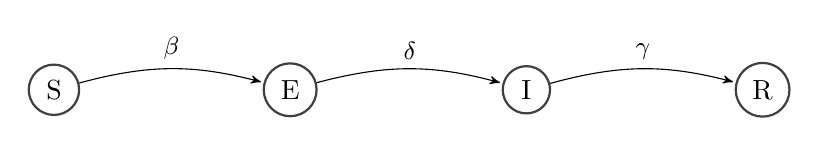
\begin{tikzpicture}[node distance=3cm,>=stealth',bend angle=15,auto]
	 	    	   \begin{scope}
	 	    	     % First net
	 	    	     \node [state] (s1)                                    {S};
	 	    	     \node [state] (s2) [right of=s1]                      {E};
	 	    	     \node [state] (s3) [right of=s2]					   {I};
	 	    	     \node [state] (s4) [right of=s3]					   {R};
	 	    	     	
	 	         	\path[every node/.style={font=\sffamily\small}]
	 	      	        (s1) edge [post, bend left] node {$\beta$} (s2)
	 	      	        (s2) edge [post, bend left] node {$\delta$} (s3)
	 	      	        (s3) edge [post, bend left] node {$\gamma$} (s4);
	 
	 	      
	 	    	   \end{scope}
	 	    	 \end{tikzpicture}
\end{figure}
\begin{description}
  \item [Exposed ($E$)] sind Individuen, welche in Kontakt mit einem Träger der Krankheit waren, aber die noch nicht infiziert sind. Die Infektion und der Ausbruch der Krankheit haben noch nicht stattgefunden, sobald dieser Zustand eintritt werden sie zu \emph{Infected}.
\end{description}
Die Übergange des Kompartimentmodells können wie folgt beschrieben werden:
 \begin{alignat*}{4}
   \frac{dS}{dt} & = - &   & \beta S I & & \\
   \frac{dE}{dt} & =   &   & \beta S I - &   & \delta E & & \\
   \frac{dI}{dt} & =   &   &  &   & \delta E - & & \gamma I \\
   \frac{dR}{dt} & =   &   &  &   &  & & \gamma I \\
 \end{alignat*}
Gekoppelt an das Ebola Beispiel können nun die Faktoren $\beta$, $\gamma$ und $\delta$ erklärt werden. Diese Faktoren können an verschiedene Krankheitsabschnitte gekoppelt werden.
\begin{description}
  \item [Kontaktrate ($\beta$)] beschreibt die Art und Weise einer Übertragung. In diesem Wert enthalten sind, die Wahrscheinlichkeit angesteckt zu werden, aber $\beta$ bildet auch das soziale Gefüge ab. Haben mehr Menschen potentiellen Kontakt zu einem Infizierten, so ist $\beta$ höher.
  \item [Inkubationsdauer ($\frac{1}{\delta}$)] beschreibt die Dauer, welche benötigt wird, bis die Krankheit in einem Individuum ausbricht.
  \item [Infektionsdauer ($\frac{1}{\gamma}$)] beschreibt die Dauer, welche die Krankheit im Körper verbleibt. Im Falle einer Genesung oder eines Exitus, ist das Individuum nicht mehr Ansteckbar. 
\end{description}
Wir verwenden die reziproken Werte $\gamma$ und $\delta$ da mit einem Zeitschlitz gerechnet wird. Wenn die Infektionsdauer 10 Tage beträgt, so ist jeden Tag die Infektion um $\frac{1}{10}$ fortgeschritten.
\begin{table}[h]
\centering
\begin{tabular}{ l r r }
						& Sierra Leone & Liberia \\
						\hline
  Kontaktrate ($\beta$) & 0.128 & 0.16 \\
  Inkubationsdauer ($\frac{1}{\delta}$) & 10 Tage & 12 Tage \\
  Infektionsdauer ($\frac{1}{\gamma}$) & 10.38 Tage & 13.31 Tage \\
\end{tabular}
\end{table}
\begin{figure}[h]
	\centering
	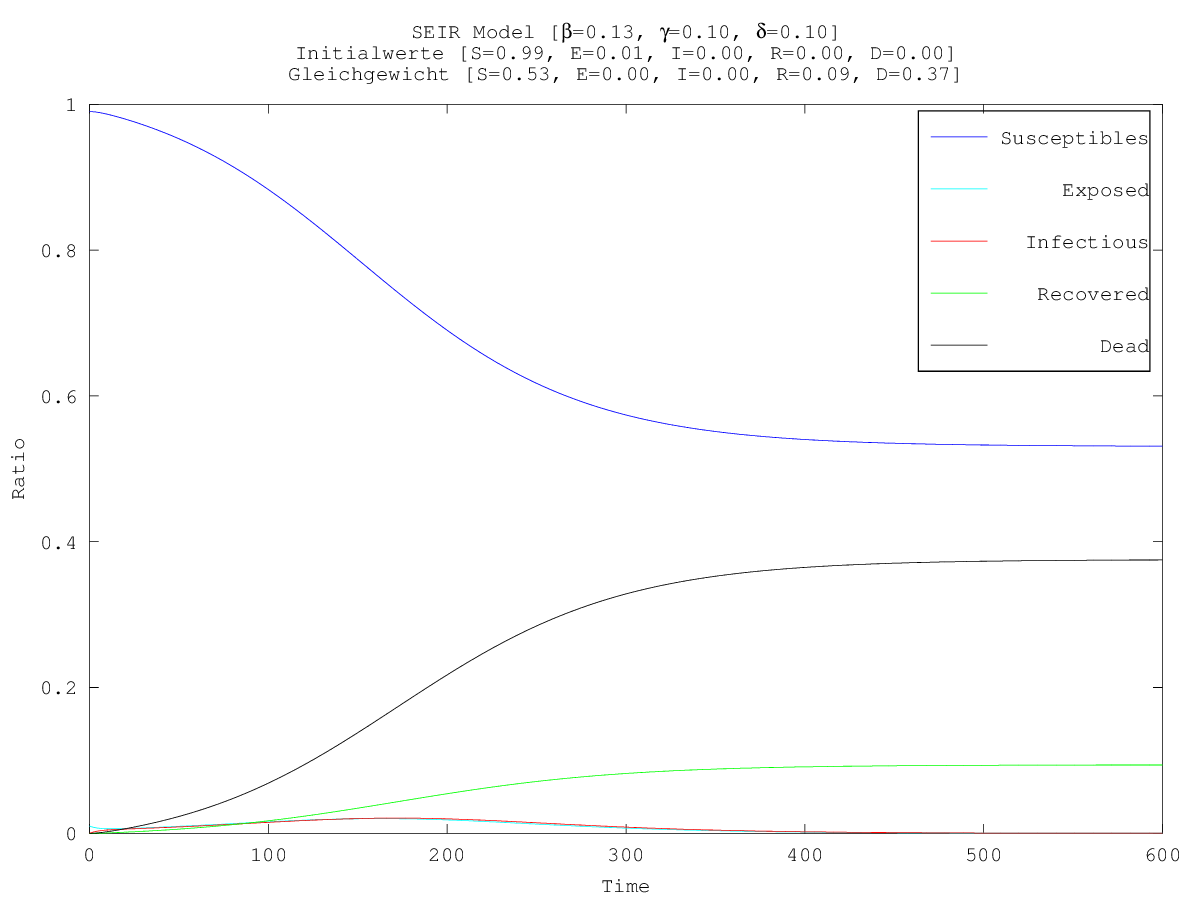
\includegraphics[width=1\textwidth]{sir/images/ebola_outbreak}
  \caption[Ebola Ausbruch]{Die Abbildung widerspiegelt den Schweregrad der Ebolaepidemie in Liberia ohne ein Eingreifen von Hilfsorganisationen, Regierungen. Da die 'Case-Fatality-Rate' (CFR) von Ebola für diese Epidemie bei 80\% liegt,\cite{sir:estimating_fatality} wurde der Vollständigkeit halber das Kompartiment $R$ (\emph{Removed}) in \emph{Recovered} und \emph{Dead} aufgeteilt.}
  \label{fig:ebola_outbreak}
\end{figure}

Wie in Abbildung~\ref{fig:ebola_outbreak} unschwer zu erkennen ist, wäre die Entwicklung in Liberia ohne dem Eingreifen der WHO fatal gewesen. Etwa 37\% der Bevölkerung wäre an den Folgen von Ebola gestorben. Doch dies war nicht der Fall. obschon sehr hohe Zahlen zu beklagen sind, sind diese nicht annähernd auf diesem erschreckend hohen Niveau. Um die Massnahmen besser zu verstehen, müssen wir zuerst verstehen, welche Parameter wirklich veränderbar sind.

Die Parameter $\gamma$ und $\delta$ sind im Grunde starre Werte, welche auch in Liberia nahezu identisch anzutreffen waren. Der einzige Parameter, welcher stark beeinflussbar sein muss, ist somit $\beta$. Der Parameter $\beta$ bildet das soziale Gefüge und die damit verbundene Wahrscheinlichkeit einer Ansteckung ab. Verschiebt sich dieser Parameter gegen 0, so werden weniger Tote zu beklagen sein, erhöht er sich jedoch, so werden massiv mehr Tote zu beklagen sein. Der Einfluss von $\beta$ auf die Mortalitätsrate ist in Abbildung~\ref{fig:beta_change_det}

\begin{figure}[h]
	\centering
	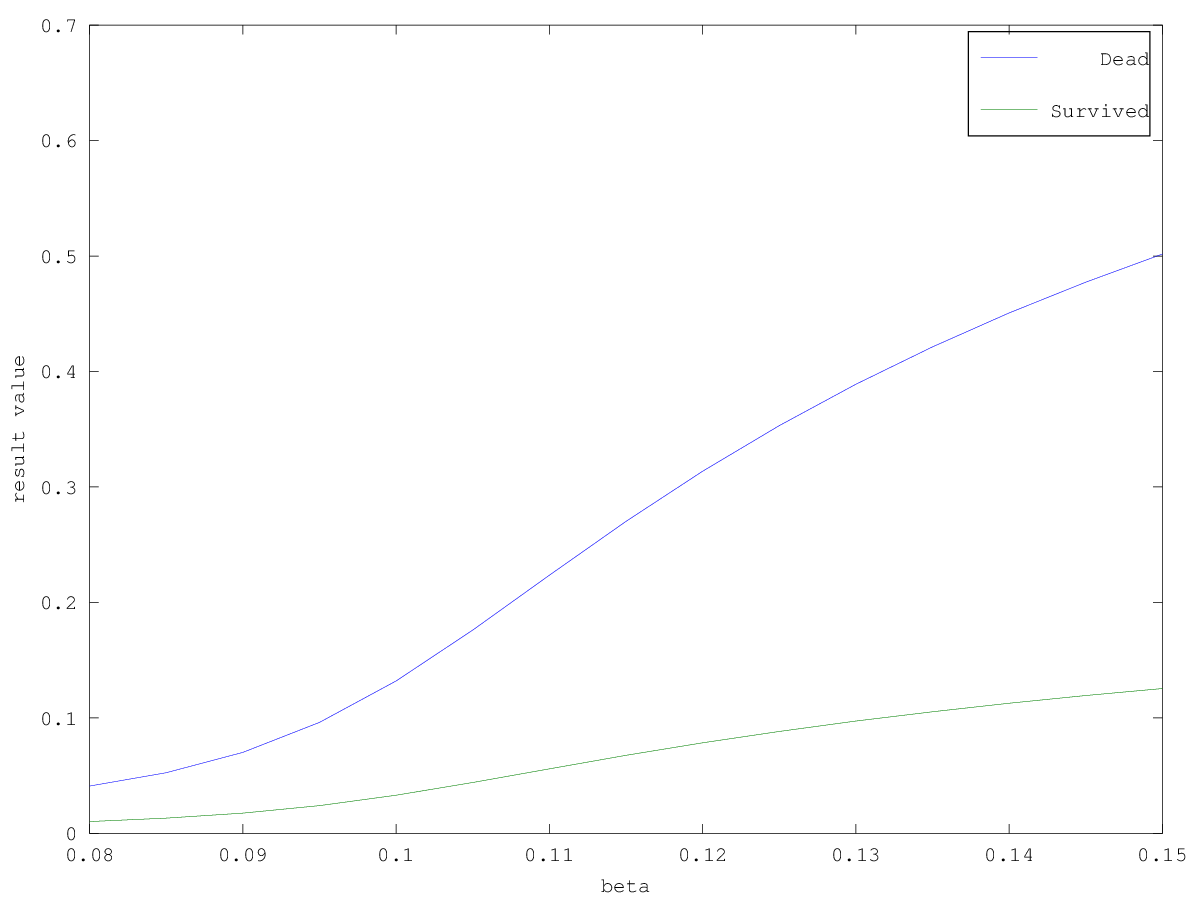
\includegraphics[width=1\textwidth]{sir/images/beta_change_det}
  \caption[Einfluss von $\beta$ auf die Mortalitätsrate]{Diese Abbildung zeigt, dass bereits eine kleine Änderungen von $\beta$ einen grossen Einfluss auf den Krankheitsverlauf hat.}
  \label{fig:beta_change_det}
\end{figure}

Die Massnahmen in Form von Quarantäne, Isolation zur Eindämmung der Krankheit, waren somit aus Sicht des Kompartimentmodelles betrachtet die richtigen Massnahmen zur Eindämmung der Krankheit, da sie effektiv die Kontaktrate $\beta$ gesenkt hatten.

\section{Zombies}
\textbf{TODO: Zombies}

\section{Weitere Anwendungsfälle}
In den bisherigen Abschnitten wurde das SIR-Modell als Grundlage für verschiedene epidemiologische Analysen zu Rate gezogen.
Es ist aber zu erwähnen, dass die zugrundeliegende Idee vom Kompartimentmodell auf viele andere Bereiche angewendet werden kann.
In der Chemie kann das Modell benutzt werden, um bei einer chemischen Reaktion zu beschreiben, wie sich der Anteil der verschiedenen Moleküle verändert, als besonders gut geeignetes Beispiel sei hier die chemische Uhr genannt.

\begin{figure}[h]
	\centering
	
\includegraphics[width=1\textwidth]{sir/images/chemical_clock}
  \caption[Chemische Uhr]{Eine chemische Uhr, ist eine chemische Reaktion, die regelmässig zwischen den zwei verschiedenen Zuständen transparent und trüb hin- und herwechselt.\cite{sir:chemical_clock}}
\end{figure}

Kompartimentmodelle können näherungsweise auch benutzt werden, um Parteizugehörigkeiten der Bevölkerung über die Zeit zu analysieren. 
Eine weitere Möglichkeit besteht auch darin, die Verbreitung von populärwissenschaftlichen Begriffen zu beschreiben. 
Ein näher mit dem hier vorgestellten SIR-Modell verwandtes Gebiet ist zum Beispiel auch die theoretische Ökologie, wobei hier der Einfluss verschiedener Populationen in der Natur zu analysieren, wie sich also eine Spezies ausbreitet oder ausstirbt.

Kompartimentmodelle können somit immer dann eingesetzt werden, wenn es darum geht, Anteile verschiedener Gruppen in einem Gesamtsystem, sowie deren Einfluss aufeinander zu modellieren. 
Damit handelt es sich um ein äusserst mächtiges Instrument in verschiedenen Bereichen. 


\printbibliography[heading=subbibliography]
\end{refsection}

